\documentclass[headsepline,toc=listof,bibliography=totocnumbered,toc=index,bibliography=oldstyle,parskip,footnotes=multiple,numbers=noendperiod,DIV=11]{scrbook}

%% BEGIN encoding
\usepackage[utf8]{inputenc}
\usepackage[ngerman]{babel}
\usepackage[T1]{fontenc}
\usepackage{lmodern}
%% END


%% BEGIN part layout
\usepackage{minitoc}
\renewcommand{\beforeparttoc}{}
\mtcsetrules{parttoc}{off}
\mtcsettitle{parttoc}{}
\doparttoc

\usepackage{scrpage2}
\renewcommand{\pagemark}{\thepart\ -\ \thepage}

\deftripstyle{PartStyle}[][]{}{}{}{}{}{\setcounter{page}{1}\setcounter{chapter}{0}}
\deftripstyle{MaintocStyle}[][]{}{}{}{}{}{\thepage}
\renewcommand*{\partpagestyle}{PartStyle}
%% END


%% BEGIN depth of numbering
\setcounter{secnumdepth}{4}    % 4 = chapter to paragraph
%% END


%% BEGIN additional useful packages
\usepackage{xspace}    % preserve spaces after commands
\usepackage{longtable} % tables over multiple pages
\usepackage{graphicx}  % include graphics
%\usepackage{psfrag}    % edit eps-graphics
%\usepackage{multicol}  % multiple (autobalanced) colums
%\usepackage{amsmath}
%\usepackage{amssymb}
%% END


%% BEGIN format links and pdf-settings
\usepackage{hyperref,breakurl}
\hyperbaseurl{.}
\hypersetup{
	colorlinks = true,
	breaklinks = true,
	citecolor = black,
	linkcolor = black,
	anchorcolor = black,
	filecolor = black,
	menucolor = black,
	urlcolor = black,
	pdfpagelayout=TwoPageRight,
	bookmarksdepth=subsection,
	pdftitle={Projekt Technische Informatik WS 2011/12 - Mini-Projekt: Minimax-Maschine},
	pdfauthor={Gerion Entrup, Martin Mattheis, Sergej Wildemann, Sven Karsten Greiner},
	pdfsubject={Projektdokumentation}
}
%% END


%% BEGIN German translations for separation-strings
\addto\extrasngerman{%
    \def\partautorefname{Teil}%
    \def\chapterautorefname{Kapitel}%
    \def\sectionautorefname{Abschnitt}%
    \def\subsectionautorefname{Abschnitt}%
    \def\subsubsectionautorefname{Abschnitt}%
    \def\paragraphautorefname{Absatz}%
    \def\figureautorefname{Abbildung}%
    \def\appendixautorefname{Anhang}%
}

\renewcommand*{\theHchapter}{\arabic{part}.\arabic{chapter}}
%% END


%% BEGIN environment for code-listings
%\usepackage[usenames]{color}
%\definecolor{BoundaryMarker}{rgb}{1,0,0}
%\definecolor{Comment}{rgb}{.5,.5,.5}
%\definecolor{Keyword}{rgb}{0,0,1}
%\definecolor{Identifier}{rgb}{0,.5,.5}
%\definecolor{Normal}{rgb}{0,0,0}
%\definecolor{String}{rgb}{0,.5,0}
%
%\usepackage{listings2}         % listings2beta because we use utf8
%\lstset{
%    language = java,
%    basicstyle = \ttfamily\fontsize{9}{11}\selectfont,
%    backgroundcolor = \color[gray]{0.95},
%    %frame = single,           % no frame because of bug in listings2beta
%    %framerule = 1pt,
%    framexleftmargin = 20pt,
%    framexrightmargin = 20pt,
%    framexbottommargin = 5pt,  % apparently no support in listings2beta
%    framextopmargin = 5pt,     % apparently no support in listings2beta
%    xleftmargin = 20pt,
%    xrightmargin = 20pt,
%    numbers = left,
%    numberstyle = \tiny,
%    numbersep = 5pt,
%    tabsize = 3,
%    breaklines = true,
%    captionpos = b,
%    firstnumber = 1,
%    stepnumber = 5,
%    breaklines = true,
%    identifierstyle=\color{Identifier},
%    commentstyle = \color{Comment},
%    keywordstyle = \color{Keyword},
%    stringstyle = \color{String}
%}
%% END


%% BEGIN create index
\makeindex
%% END


%% BEGIN helper for titlepage
\newcommand{\maketitlepage}{
    \subject{Projekt Technische Informatik WS 2011/12}
    \title{Mini-Projekt:\\ Minimax-Maschine}
    \author{Gerion Entrup\\ Martin Mattheis\\ Sergej Wildemann\\ Sven Karsten Greiner}
    \date{\today}
    
    \maketitle
}
%% END


%% BEGIN helper for main table of contents
\newcommand{\makemaintoc}{
    \cleardoublepage
    \begingroup
        \pagestyle{MaintocStyle}
        \renewcommand*{\chapterpagestyle}{MaintocStyle}
        
        \pagenumbering{roman}
        
        \setcounter{tocdepth}{0}
        \tableofcontents
        
        \cleardoublepage
    \endgroup
    \pagenumbering{arabic}
}
%% END


%% BEGIN helper for TODO
\newcommand{\todo}[1]{%
    \marginpar{%
        \colorbox{red}{%
            \parbox{\marginparwidth}{%
                \color{white}
                \tiny
                \raggedright
                #1
            }
        }
    }
}
%% END


%% BEGIN helper for glossar
\newcommand{\glsentry}[2]{
   \textbf{#1}
   \begingroup
      \setlength{\parskip}{0pt}
      \begin{addmargin}[2em]{}
         #2
      \end{addmargin}
   \endgroup
}
%% END


%% BEGIN no hyphenation for listed words (CSV)
\hyphenation{}
%% END


%% BEGIN document
\begin{document}

%% BEGIN title and table of contents
\maketitlepage
\makemaintoc
%% END


%% BEGIN content
\part{Pflichtenheft}
\label{part:Pflichtenheft}

\parttoc

\chapter{Einführung}
\label{chapter:Dokumentation-Einfuehrung}

Im Folgenden wird der Algorithmus aus \autoref{subsection:Pflichtenheft-SystemtechnischeLoesung-Loesungsansatz-Ansatz2} von \autoref{part:Pflichtenheft} konkretisiert und implementiert.

Dazu wird die Konfigurationsdatei für die nötige Hardwareerweiterung erstellt. Parallel dazu wird der Algorithmus auf Basis des Flussdiagramms zuerst in Pseudocode verfasst, welcher danach in die RT"=Notation übertragen wird. Diese RT"=Notation wird anschließend in eine Steuertabelle für die Minimax"=Maschine übersetzt.\\
Eine genauere Beschreibung inklusive Ergebnisse befindet sich in \autoref{chapter:Dokumentation-Implementierung}, der Code im Anhang (\autoref{part:Anhang}).

Mit diesen Vorbereitungen kann der Simulator gestartet werden. Eine Erläuterung befindet sich in \autoref{chapter:Dokumentation-Simulation}.

Abschließend wird das Ergebnis in \autoref{chapter:Dokumentation-BenchmarkBewertung} analysiert und bewertet.


\section{Protokollierung}
\label{section:Dokumentation-Einfuehrung-Protokollierung}

\begin{tabularx}{\textwidth}{|l|l|X|c|}
    \hline
    Datum & Bearbeiter & Vorgang & Zeit \\
    \hline
    \hline
    10.01.2012 & Wildemann & Grundentwurf für Algorithmus, Pseudocode, Abstraktion, Diagramm & 2,5 h \\
    \hline
    16.01.2012 & Greiner & Grundgerüst für Dokumentation & 1 h \\
    \hline
    18.01.2012 & Entrup, Wildemann & Simulator analysiert, Workarounds für Probleme gesucht & 3 h \\
    \hline
    19.01.2012 & Entrup, Wildemann & RT"=Notation & 2 h\\
    \hline
    20.01.2012 & Matthaei, Wildemann & Steuertabelle & 3 h\\
    \hline
    22.01.2012 & alle & Tests und Korrekturen & 10 h\\
    \hline
    23.01.2012 & Wildemann & Optimierungen & 1,5 h \\
               & alle & Tests, Korrekturen, Benchmarkberechnung, Aufräumen & 5 h \\
               & Greiner & Aktualisierung der Dokumentation & 1,5 h \\
    \hline
\end{tabularx}

\chapter{Istzustand}
\label{chapter:Pflichtenheft-Istzustand}

\section{Der Simulator}
\label{section:Pflichtenheft-Istzustand-Simulator}

Vom Auftraggeber ist ein lauffähiger Simulator einer Minimax"=Maschine gegeben. Dieser wird über Textdateien gesteuert, welche die Hardwarekomponenten in einer speziellen Beschreibungssprache definieren. Dazu zählen unter anderem Register, Multiplexer, ALU, CU, Sign, Speicher und Verbindungen. Durch hinzufügen weiterer Steuerungsdateien lässt sich die virtuelle Maschine erweitern.

Der Simulator selbst ist in Java (ab 1.3) realisiert und somit plattformunabhängig. Ein Quellcode liegt nicht vor.

Begleitend ist ein umfangreiches Handbuch in PDF"=Form vorhanden (siehe \cite{minimax-handbuch}), welches alle wichtigen Eigenschaften des Simulators und der Basiskonfiguration erläutert. Weitere Informationen zum Simulator können diesem entnommen werden. Für die Bedienung notwendige Schritte werden später in \autoref{part:Dokumentation} dieser Dokumentation erläutert.

\begin{figure}[htb]
    \centering
    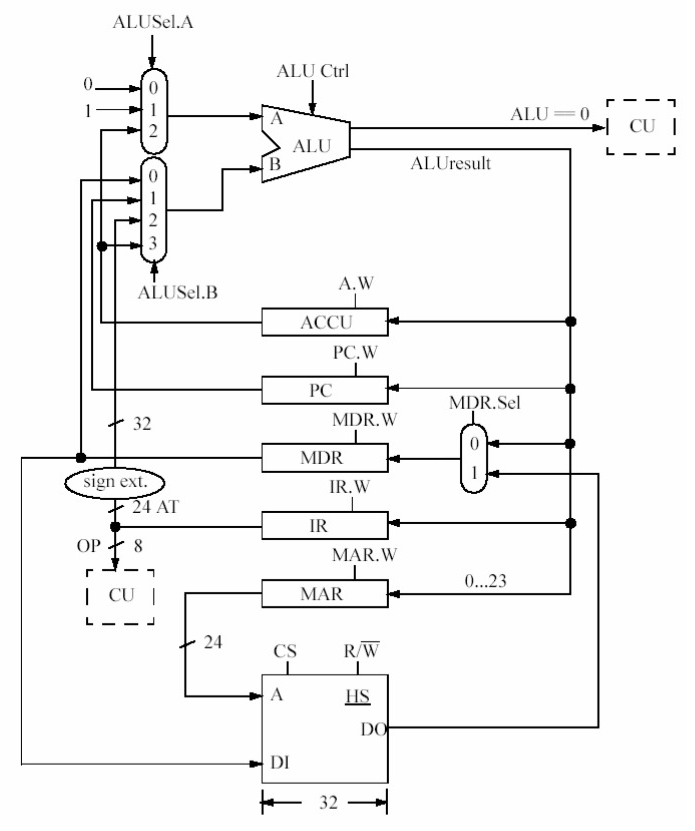
\includegraphics[width=0.7\textwidth]{pflichtenheft/res/minimax.png}
    \caption{Schematische Darstellung der Minimax"=Maschine}
    \label{figure:Pflichtenheft-Istzustand-Simulator-Schema}
\end{figure}

Im Folgenden soll noch die gegebene Basiskonfiguration erläutert werden.

\subsection{Basiskonfiguration}
\label{subsection:Pflichtenheft-Istzustand-Simulator-Basiskonfiguration}

Die Minimax"=Maschine arbeitet vereinfacht ausgedrückt mit einem Datenkreislauf zwischen \emph{Registern} und der \emph{Arithmetic Logic Unit} (ALU), gesteuert durch die \emph{Control Unit} (CU). In der Basiskonfiguration existieren folgende Register (mit ihren jeweilig zugedachten Aufgaben):

\begin{description}
    \item[ACCU] \emph{Accumulator}, Zwischenspeicher
    \item[PC] \emph{Program Counter}, Zähler für Programmablauf
    \item[MDR] \emph{Memory Data Register}, erhält Daten gesteuert durch den Multiplexer \emph{MDR.Sel} (MDR Selector) entweder aus der ALU oder aus dem Hauptspeicher (HS)
    \item[IR] \emph{Instruction Register}, enthält den aktuellen Befehl (8 Bit) mit Adressteil \emph{AT} (24 Bit). Der Befehl wird an die CU weitergeleitet. Der Adressteil wird durch die Sign Extension Unit vorzeichenrichtig auf 32 Bit aufgefüllt.\todo{verschönern}
    \item[MAR] \emph{Memory Address Register}, enthält die Speicheradresse, aus der Daten vom HS gelesen werden sollen
\end{description}

Jedes Register hat als Eingang mindestens die ALU und besitzt zusätlich einen Steuerungseingang, welcher den Schreibzugriff regelt.

Die ALU wird über den Eingang \emph{ALU.Ctrl} gesteuert und  hat zwei Eingänge, welche mit Multiplexern (gesteuert über \emph{ALUSel.A} und \emph{ALUSel.B}) beschaltet sind. Diese haben folgende Eingänge:

\textbf{A:} 0, 1, ACCU\\
\textbf{B:} MDR, PC, AT, ACCU

In der ALU sind durch die Basiskonfiguration folgende Operationen implementiert:

\begin{description}
    \item[ADD] $ALUresult \gets A + B$
    \item[SUB.B] $ALUresult \gets -A + B$
    \item[TRANS.A] $ALUresult \gets A$
    \item[TRANS.B] $ALUresult \gets B$
\end{description}

\todo{
\begin{itemize}
    \item Speicherbreite
    \item Speicherzugriff
    \item CU, PC genauer erläutern
\end{itemize}
}


\section{Projektdateien}
\label{section:Pflichtenheft-Istzustand-Projektdateien}

Die Aufgaben und Anforderungen wurden als PDF"=Dokument (siehe \cite{aufgabenblatt}) zur Verfügung gestellt. Einige Punkte daraus werden bei Gelegenheit in diesem Dokument aufgeführt und erläutert. Weitere Informationen zum Projekt befinden sich in einer weiteren PDF (siehe \cite{projektinfo}).

In Bezug auf die Aufgabe sind außerdem Speicherabbilder für einen einheitlichen Benchmark"=Vergleich gegeben. Das Format kann vom Simulator ohne Anpassungen gelesen werden.


\chapter[Sollzustand]{Sollzustand\footnote{Größtenteils übernommen aus \cite{aufgabenblatt}}}
\label{chapter:Pflichtenheft-Sollzustand}

Im Hauptspeicher der Minimax"=Machine sind unterschiedliche Datenpakete abgelegt. Jedes Paket enthält einen Kopf von 80 Bits und einen Datenteil mit variabler Länge. Ein Paket fängt mit dem festgelegten Muster \texttt{1110} an. Innerhalb des Kopfes ist die Kanalnummer in zwei nacheinander folgenden Bytes ab dem Bit Nummer 32 vertretet. Zu einem Kanal können mehrere Pakete mit einer eindeutigen Kanalnummer gehören.

\begin{center}
    \begin{tabular}{|c|c|c|c|c|}
        \multicolumn{1}{c}{0-3} & \multicolumn{1}{c}{} & \multicolumn{1}{c}{32-47} & \multicolumn{1}{c}{48-79} & \multicolumn{1}{c}{} \\
        \hline
        1110 & xxx & Kanalnummer & xxx & \hspace{1cm} Datenteil \hspace{1cm} \\
        \hline
    \end{tabular}
\end{center}

\begin{center}
    \begin{tabular}{|c|c|c|c|c|c|c|c|c|}
        \hline
        H_0 & \hspace{.3cm} D_0 \hspace*{.3cm} & H_1 & D_1 & H_2 & \hspace{1cm} D_2 \hspace*{1cm} & ...... & H_n & D_n \\
        \hline
    \end{tabular}
\end{center}

Es soll ein Algorithmus entwickelt und mit der Minimax"=Maschine implementiert werden, welcher eine Speichertabelle der Kanalnummern und der Länge (in Bits) des Datenteils aller Pakete des jeweiligen Kanals erstellt. Diese Tabelle soll an einer beliebigen Stelle im Hauptspeicher (außerhalb des Paketfeldbereiches) abgelegt werden.

Beim Aufruf des Algorithmus wird dem Befehl die Länge des Paketfeldes übergeben. Der ACCU beinhaltet bereits die Speicheradresse, an welcher das Paketfeld beginnt.

\pagebreak

Wenn z.\,B. die Datentabelle so aussieht:

\begin{center}
    \begin{tabular}{|c|c|c|c|c|c|c|c|c|c|c|c|c|c|c|}
        \multicolumn{5}{c|}{1. Paket} & \multicolumn{5}{c|}{2. Paket} & \multicolumn{5}{c}{3. Paket}\\ \hline
        1110 & x & $243_{10}$ & x & 1001 & 1110 & x & $243_{10}$ & x & 10110 & 1110 & x & $3727_{10}$ & x & 1001 \\ \hline
    \end{tabular}
\end{center}

ergibt sich daraus folgende Tabelle:

\begin{center}
    \begin{tabular}{|r|r|l|}
        \hline
        Kanalnr. & Anzahl \\
        \hline
        \hline
        243 & 9 \\
        \hline
        3727 & 4 \\
        \hline
    \end{tabular}
\end{center}

\chapter{Systemtechnische Lösung}
\label{chapter:Pflichtenheft-SystemtechnischeLoesung}

\section{Lösungsansatz}
\label{section:Pflichtenheft-SystemtechnischeLoesung-Loesungsansatz}

Die erste Schritt ist zu klären, wie die Tabelle im Speicher gespeichert werden soll. Dabei gilt zu beachten, dass unbegrenzt Speicher vorhanden ist und keine Bewertung hinsichtlich des Speichers getroffen wird.

\subsection{Ansatz 1}
Man speichert die Kanalnummer in Register x und die herausgefundene Anzahl Datenbits, die zu dieser Kanalnummer gehören, in Register x+1.

Vorteile:
\begin{itemize}
    \item Man findet sehr schnell zu einer Kanalnummer die entsprechende Anzahl.
    \item Geringer Speicherverbrauch.
\end{itemize}

Nachteile:
\begin{itemize}
    \item Die Kanalnummern werden sehr langsam gefunden, es sei denn man sortiert sie.
    \item Wenn man die Kanalnummern sortiert, muss man die höheren nach hinten verschieben.
\end{itemize}

\subsection{Ansatz 2}
Man speichert in dem Register mit der Kanalnummer (plus einem Offset) die herausgefundene Anzahl Datenbits, die zu dieser Kanalnummer gehören.

Vorteile:
\begin{itemize}
    \item Sehr schnelle Berechnung des Registers, in dem die gewünschte Anzahl steht.
    \item Keine Sortierung notwendig.
    \item Reduzierung des Nettospeicherverbrauchs.
\end{itemize}

Nachteile:
\begin{itemize}
    \item Hoher Bruttospeicherverbrauch, da viele mögliche Nummer unnutzbaren Speicher darstellen.
    \item Schlecht "`per Auge"' ablesbar, weil man die Registernummer berechnen muss.
\end{itemize}

Wir haben uns wegen der sehr umständlichen Speicheroperationen gegen den ersten Ansatz entschieden.

Da man nur 32 bits auf einmal auslesen kann, muss man mit der Alu die Operation "`shift"' hinzufügen. Der Offset wird als die Länge des Datenteils festgelegt.\\
Der Algorithmus sieht dann so aus:
\todo{flussdiagramm}

\todo{zwei Ansätze, beide kurz erläutern, sich auf einen festlegen (mit Begründung) und ggf. weiter vertiefen.}


\section{Gliederung}
\label{section:Pflichtenheft-SystemtechnischeLoesung-Gliederung}

\todo{Schilderung des Ablaufs der weiteren Entwicklung nach Auftragserteilung. Arbeitszuweisung, Zeitplan, benötigte Ressourcen etc.}


\section{Regulärer Betrieb}
\label{section:Pflichtenheft-SystemtechnischeLoesung-regulaer}

Nach Aufruf des Alorithmus mit korrekten Startparametern (siehe \autoref{chapter:Pflichtenheft-Sollzustand}), läuft dieser solange, bis er nach Erreichen der gegebenen Länge des Datenblockfelds terminiert. Im Hauptspeicher liegt dann eine Tabelle der Kanalnummern und ihrer jeweiligen Datenlänge vor.


\section{Irregulärer Betrieb}
\label{section:Pflichtenheft-SystemtechnischeLoesung-irregulaer}

Eine Reihe von Ereignissen kann zu einem fehlerhaften Verhalten des Algorithmus führen.
\todo{Terminiert der Algorithmus nicht immer, da er die Länge des Datenfeldes gegeben bekommt?}

\subsection{Fehlerhafte Startparameter}
\label{subsection:Pflichtenheft-SystemtechnischeLoesung-irregulaer-startparameter}

Es kann sein, dass der übergebene Parameter nicht den korrekten Beginn des Datenfeldes beschreibt. In diesem Fall ist nicht vorherzusehen, wie sich der Algorithmus verhält. Man kann allerdings überprüfen, ob der Beginn mit dem Startcode \texttt{1110} beginnt und diesen Fehlerfall somit weitgehend vermeiden.

Falls die angegebene Länge nicht zu den Daten im Hauptspeicher passt, wird entweder ein Teil der Daten vernachlässigt oder undefinierter Speicherinhalt gelesen und dem Ergebnis hinzugefügt. Dies verfälscht zwar das Ergebnis, lässt den Algorithmus jedoch korrekt terminieren, sofern der Code \texttt{1110} nicht im undefinierten Teil vorkommt (siehe \autoref{subsection:Pflichtenheft-SystemtechnischeLoesung-irregulaer-syntax}).

\subsection{Fehlerhafte Datensyntax}
\label{subsection:Pflichtenheft-SystemtechnischeLoesung-irregulaer-syntax}

Jedes Paket beginnt mit dem Muster \texttt{1110} (vgl. \autoref{chapter:Pflichtenheft-Sollzustand}). Sollte dieses Muster unerwartet \emph{nicht} als Beginn eines Pakets auftreten, arbeitet der Algorithmus undefiniert weiter, bis er wieder auf ein neues Paket mit korrekter Syntax trifft.

Laut Definition der Daten kann \texttt{1110} jedoch nicht an einer solchen falschen Stelle auftreten. Einzige Möglichkeit wäre demzufolge ein fehlerhafter Einsatz des Algorithmus oder eine Beschädigung des Datenfeldes.

\subsection{Modifikation des Datenfeldes während der Laufzeit}
\label{subsection:Pflichtenheft-SystemtechnischeLoesung-irregulaer-moddatenfeld}

Findet während der Laufzeit eine Modifikation des Datenfeldes statt, welches bereits abgearbeitet wurde, so ändert dies das Ergebnis nicht. Eine Modifikation des kommenden Teils führt zu einem verfälschtem Ergebnis oder nach \autoref{subsection:Pflichtenheft-SystemtechnischeLoesung-irregulaer-syntax} zu einem undefinierten Zustand.

\subsection{Modifikation des Tabellenteils während der Laufzeit}
\label{subsection:Pflichtenheft-SystemtechnischeLoesung-irregulaer-modtabelle}

Eine Modifikation der Ergebnistabelle während der Laufzeit führt zu fehlerhaften Datenlängen. \todo{Wenn wir die Daten nicht mit der Kanalnummer adressieren, kann die komplette Datenstruktur zerstört werden.}



\part{Pflichtenheft}
\label{part:Pflichtenheft}

\parttoc

\chapter{Einführung}
\label{chapter:Dokumentation-Einfuehrung}

Im Folgenden wird der Algorithmus aus \autoref{subsection:Pflichtenheft-SystemtechnischeLoesung-Loesungsansatz-Ansatz2} von \autoref{part:Pflichtenheft} konkretisiert und implementiert.

Dazu wird die Konfigurationsdatei für die nötige Hardwareerweiterung erstellt. Parallel dazu wird der Algorithmus auf Basis des Flussdiagramms zuerst in Pseudocode verfasst, welcher danach in die RT"=Notation übertragen wird. Diese RT"=Notation wird anschließend in eine Steuertabelle für die Minimax"=Maschine übersetzt.\\
Eine genauere Beschreibung inklusive Ergebnisse befindet sich in \autoref{chapter:Dokumentation-Implementierung}, der Code im Anhang (\autoref{part:Anhang}).

Mit diesen Vorbereitungen kann der Simulator gestartet werden. Eine Erläuterung befindet sich in \autoref{chapter:Dokumentation-Simulation}.

Abschließend wird das Ergebnis in \autoref{chapter:Dokumentation-BenchmarkBewertung} analysiert und bewertet.


\section{Protokollierung}
\label{section:Dokumentation-Einfuehrung-Protokollierung}

\begin{tabularx}{\textwidth}{|l|l|X|c|}
    \hline
    Datum & Bearbeiter & Vorgang & Zeit \\
    \hline
    \hline
    10.01.2012 & Wildemann & Grundentwurf für Algorithmus, Pseudocode, Abstraktion, Diagramm & 2,5 h \\
    \hline
    16.01.2012 & Greiner & Grundgerüst für Dokumentation & 1 h \\
    \hline
    18.01.2012 & Entrup, Wildemann & Simulator analysiert, Workarounds für Probleme gesucht & 3 h \\
    \hline
    19.01.2012 & Entrup, Wildemann & RT"=Notation & 2 h\\
    \hline
    20.01.2012 & Matthaei, Wildemann & Steuertabelle & 3 h\\
    \hline
    22.01.2012 & alle & Tests und Korrekturen & 10 h\\
    \hline
    23.01.2012 & Wildemann & Optimierungen & 1,5 h \\
               & alle & Tests, Korrekturen, Benchmarkberechnung, Aufräumen & 5 h \\
               & Greiner & Aktualisierung der Dokumentation & 1,5 h \\
    \hline
\end{tabularx}

\chapter{Istzustand}
\label{chapter:Pflichtenheft-Istzustand}

\section{Der Simulator}
\label{section:Pflichtenheft-Istzustand-Simulator}

Vom Auftraggeber ist ein lauffähiger Simulator einer Minimax"=Maschine gegeben. Dieser wird über Textdateien gesteuert, welche die Hardwarekomponenten in einer speziellen Beschreibungssprache definieren. Dazu zählen unter anderem Register, Multiplexer, ALU, CU, Sign, Speicher und Verbindungen. Durch hinzufügen weiterer Steuerungsdateien lässt sich die virtuelle Maschine erweitern.

Der Simulator selbst ist in Java (ab 1.3) realisiert und somit plattformunabhängig. Ein Quellcode liegt nicht vor.

Begleitend ist ein umfangreiches Handbuch in PDF"=Form vorhanden (siehe \cite{minimax-handbuch}), welches alle wichtigen Eigenschaften des Simulators und der Basiskonfiguration erläutert. Weitere Informationen zum Simulator können diesem entnommen werden. Für die Bedienung notwendige Schritte werden später in \autoref{part:Dokumentation} dieser Dokumentation erläutert.

\begin{figure}[htb]
    \centering
    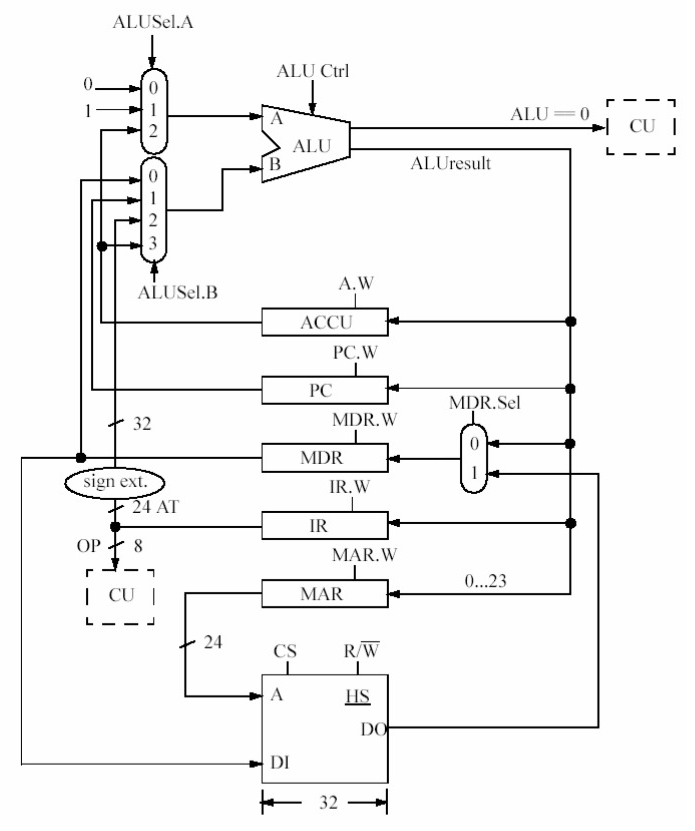
\includegraphics[width=0.7\textwidth]{pflichtenheft/res/minimax.png}
    \caption{Schematische Darstellung der Minimax"=Maschine}
    \label{figure:Pflichtenheft-Istzustand-Simulator-Schema}
\end{figure}

Im Folgenden soll noch die gegebene Basiskonfiguration erläutert werden.

\subsection{Basiskonfiguration}
\label{subsection:Pflichtenheft-Istzustand-Simulator-Basiskonfiguration}

Die Minimax"=Maschine arbeitet vereinfacht ausgedrückt mit einem Datenkreislauf zwischen \emph{Registern} und der \emph{Arithmetic Logic Unit} (ALU), gesteuert durch die \emph{Control Unit} (CU). In der Basiskonfiguration existieren folgende Register (mit ihren jeweilig zugedachten Aufgaben):

\begin{description}
    \item[ACCU] \emph{Accumulator}, Zwischenspeicher
    \item[PC] \emph{Program Counter}, Zähler für Programmablauf
    \item[MDR] \emph{Memory Data Register}, erhält Daten gesteuert durch den Multiplexer \emph{MDR.Sel} (MDR Selector) entweder aus der ALU oder aus dem Hauptspeicher (HS)
    \item[IR] \emph{Instruction Register}, enthält den aktuellen Befehl (8 Bit) mit Adressteil \emph{AT} (24 Bit). Der Befehl wird an die CU weitergeleitet. Der Adressteil wird durch die Sign Extension Unit vorzeichenrichtig auf 32 Bit aufgefüllt.\todo{verschönern}
    \item[MAR] \emph{Memory Address Register}, enthält die Speicheradresse, aus der Daten vom HS gelesen werden sollen
\end{description}

Jedes Register hat als Eingang mindestens die ALU und besitzt zusätlich einen Steuerungseingang, welcher den Schreibzugriff regelt.

Die ALU wird über den Eingang \emph{ALU.Ctrl} gesteuert und  hat zwei Eingänge, welche mit Multiplexern (gesteuert über \emph{ALUSel.A} und \emph{ALUSel.B}) beschaltet sind. Diese haben folgende Eingänge:

\textbf{A:} 0, 1, ACCU\\
\textbf{B:} MDR, PC, AT, ACCU

In der ALU sind durch die Basiskonfiguration folgende Operationen implementiert:

\begin{description}
    \item[ADD] $ALUresult \gets A + B$
    \item[SUB.B] $ALUresult \gets -A + B$
    \item[TRANS.A] $ALUresult \gets A$
    \item[TRANS.B] $ALUresult \gets B$
\end{description}

\todo{
\begin{itemize}
    \item Speicherbreite
    \item Speicherzugriff
    \item CU, PC genauer erläutern
\end{itemize}
}


\section{Projektdateien}
\label{section:Pflichtenheft-Istzustand-Projektdateien}

Die Aufgaben und Anforderungen wurden als PDF"=Dokument (siehe \cite{aufgabenblatt}) zur Verfügung gestellt. Einige Punkte daraus werden bei Gelegenheit in diesem Dokument aufgeführt und erläutert. Weitere Informationen zum Projekt befinden sich in einer weiteren PDF (siehe \cite{projektinfo}).

In Bezug auf die Aufgabe sind außerdem Speicherabbilder für einen einheitlichen Benchmark"=Vergleich gegeben. Das Format kann vom Simulator ohne Anpassungen gelesen werden.


\chapter[Sollzustand]{Sollzustand\footnote{Größtenteils übernommen aus \cite{aufgabenblatt}}}
\label{chapter:Pflichtenheft-Sollzustand}

Im Hauptspeicher der Minimax"=Machine sind unterschiedliche Datenpakete abgelegt. Jedes Paket enthält einen Kopf von 80 Bits und einen Datenteil mit variabler Länge. Ein Paket fängt mit dem festgelegten Muster \texttt{1110} an. Innerhalb des Kopfes ist die Kanalnummer in zwei nacheinander folgenden Bytes ab dem Bit Nummer 32 vertretet. Zu einem Kanal können mehrere Pakete mit einer eindeutigen Kanalnummer gehören.

\begin{center}
    \begin{tabular}{|c|c|c|c|c|}
        \multicolumn{1}{c}{0-3} & \multicolumn{1}{c}{} & \multicolumn{1}{c}{32-47} & \multicolumn{1}{c}{48-79} & \multicolumn{1}{c}{} \\
        \hline
        1110 & xxx & Kanalnummer & xxx & \hspace{1cm} Datenteil \hspace{1cm} \\
        \hline
    \end{tabular}
\end{center}

\begin{center}
    \begin{tabular}{|c|c|c|c|c|c|c|c|c|}
        \hline
        H_0 & \hspace{.3cm} D_0 \hspace*{.3cm} & H_1 & D_1 & H_2 & \hspace{1cm} D_2 \hspace*{1cm} & ...... & H_n & D_n \\
        \hline
    \end{tabular}
\end{center}

Es soll ein Algorithmus entwickelt und mit der Minimax"=Maschine implementiert werden, welcher eine Speichertabelle der Kanalnummern und der Länge (in Bits) des Datenteils aller Pakete des jeweiligen Kanals erstellt. Diese Tabelle soll an einer beliebigen Stelle im Hauptspeicher (außerhalb des Paketfeldbereiches) abgelegt werden.

Beim Aufruf des Algorithmus wird dem Befehl die Länge des Paketfeldes übergeben. Der ACCU beinhaltet bereits die Speicheradresse, an welcher das Paketfeld beginnt.

\pagebreak

Wenn z.\,B. die Datentabelle so aussieht:

\begin{center}
    \begin{tabular}{|c|c|c|c|c|c|c|c|c|c|c|c|c|c|c|}
        \multicolumn{5}{c|}{1. Paket} & \multicolumn{5}{c|}{2. Paket} & \multicolumn{5}{c}{3. Paket}\\ \hline
        1110 & x & $243_{10}$ & x & 1001 & 1110 & x & $243_{10}$ & x & 10110 & 1110 & x & $3727_{10}$ & x & 1001 \\ \hline
    \end{tabular}
\end{center}

ergibt sich daraus folgende Tabelle:

\begin{center}
    \begin{tabular}{|r|r|l|}
        \hline
        Kanalnr. & Anzahl \\
        \hline
        \hline
        243 & 9 \\
        \hline
        3727 & 4 \\
        \hline
    \end{tabular}
\end{center}

\chapter{Systemtechnische Lösung}
\label{chapter:Pflichtenheft-SystemtechnischeLoesung}

\section{Lösungsansatz}
\label{section:Pflichtenheft-SystemtechnischeLoesung-Loesungsansatz}

Die erste Schritt ist zu klären, wie die Tabelle im Speicher gespeichert werden soll. Dabei gilt zu beachten, dass unbegrenzt Speicher vorhanden ist und keine Bewertung hinsichtlich des Speichers getroffen wird.

\subsection{Ansatz 1}
Man speichert die Kanalnummer in Register x und die herausgefundene Anzahl Datenbits, die zu dieser Kanalnummer gehören, in Register x+1.

Vorteile:
\begin{itemize}
    \item Man findet sehr schnell zu einer Kanalnummer die entsprechende Anzahl.
    \item Geringer Speicherverbrauch.
\end{itemize}

Nachteile:
\begin{itemize}
    \item Die Kanalnummern werden sehr langsam gefunden, es sei denn man sortiert sie.
    \item Wenn man die Kanalnummern sortiert, muss man die höheren nach hinten verschieben.
\end{itemize}

\subsection{Ansatz 2}
Man speichert in dem Register mit der Kanalnummer (plus einem Offset) die herausgefundene Anzahl Datenbits, die zu dieser Kanalnummer gehören.

Vorteile:
\begin{itemize}
    \item Sehr schnelle Berechnung des Registers, in dem die gewünschte Anzahl steht.
    \item Keine Sortierung notwendig.
    \item Reduzierung des Nettospeicherverbrauchs.
\end{itemize}

Nachteile:
\begin{itemize}
    \item Hoher Bruttospeicherverbrauch, da viele mögliche Nummer unnutzbaren Speicher darstellen.
    \item Schlecht "`per Auge"' ablesbar, weil man die Registernummer berechnen muss.
\end{itemize}

Wir haben uns wegen der sehr umständlichen Speicheroperationen gegen den ersten Ansatz entschieden.

Da man nur 32 bits auf einmal auslesen kann, muss man mit der Alu die Operation "`shift"' hinzufügen. Der Offset wird als die Länge des Datenteils festgelegt.\\
Der Algorithmus sieht dann so aus:
\todo{flussdiagramm}

\todo{zwei Ansätze, beide kurz erläutern, sich auf einen festlegen (mit Begründung) und ggf. weiter vertiefen.}


\section{Gliederung}
\label{section:Pflichtenheft-SystemtechnischeLoesung-Gliederung}

\todo{Schilderung des Ablaufs der weiteren Entwicklung nach Auftragserteilung. Arbeitszuweisung, Zeitplan, benötigte Ressourcen etc.}


\section{Regulärer Betrieb}
\label{section:Pflichtenheft-SystemtechnischeLoesung-regulaer}

Nach Aufruf des Alorithmus mit korrekten Startparametern (siehe \autoref{chapter:Pflichtenheft-Sollzustand}), läuft dieser solange, bis er nach Erreichen der gegebenen Länge des Datenblockfelds terminiert. Im Hauptspeicher liegt dann eine Tabelle der Kanalnummern und ihrer jeweiligen Datenlänge vor.


\section{Irregulärer Betrieb}
\label{section:Pflichtenheft-SystemtechnischeLoesung-irregulaer}

Eine Reihe von Ereignissen kann zu einem fehlerhaften Verhalten des Algorithmus führen.
\todo{Terminiert der Algorithmus nicht immer, da er die Länge des Datenfeldes gegeben bekommt?}

\subsection{Fehlerhafte Startparameter}
\label{subsection:Pflichtenheft-SystemtechnischeLoesung-irregulaer-startparameter}

Es kann sein, dass der übergebene Parameter nicht den korrekten Beginn des Datenfeldes beschreibt. In diesem Fall ist nicht vorherzusehen, wie sich der Algorithmus verhält. Man kann allerdings überprüfen, ob der Beginn mit dem Startcode \texttt{1110} beginnt und diesen Fehlerfall somit weitgehend vermeiden.

Falls die angegebene Länge nicht zu den Daten im Hauptspeicher passt, wird entweder ein Teil der Daten vernachlässigt oder undefinierter Speicherinhalt gelesen und dem Ergebnis hinzugefügt. Dies verfälscht zwar das Ergebnis, lässt den Algorithmus jedoch korrekt terminieren, sofern der Code \texttt{1110} nicht im undefinierten Teil vorkommt (siehe \autoref{subsection:Pflichtenheft-SystemtechnischeLoesung-irregulaer-syntax}).

\subsection{Fehlerhafte Datensyntax}
\label{subsection:Pflichtenheft-SystemtechnischeLoesung-irregulaer-syntax}

Jedes Paket beginnt mit dem Muster \texttt{1110} (vgl. \autoref{chapter:Pflichtenheft-Sollzustand}). Sollte dieses Muster unerwartet \emph{nicht} als Beginn eines Pakets auftreten, arbeitet der Algorithmus undefiniert weiter, bis er wieder auf ein neues Paket mit korrekter Syntax trifft.

Laut Definition der Daten kann \texttt{1110} jedoch nicht an einer solchen falschen Stelle auftreten. Einzige Möglichkeit wäre demzufolge ein fehlerhafter Einsatz des Algorithmus oder eine Beschädigung des Datenfeldes.

\subsection{Modifikation des Datenfeldes während der Laufzeit}
\label{subsection:Pflichtenheft-SystemtechnischeLoesung-irregulaer-moddatenfeld}

Findet während der Laufzeit eine Modifikation des Datenfeldes statt, welches bereits abgearbeitet wurde, so ändert dies das Ergebnis nicht. Eine Modifikation des kommenden Teils führt zu einem verfälschtem Ergebnis oder nach \autoref{subsection:Pflichtenheft-SystemtechnischeLoesung-irregulaer-syntax} zu einem undefinierten Zustand.

\subsection{Modifikation des Tabellenteils während der Laufzeit}
\label{subsection:Pflichtenheft-SystemtechnischeLoesung-irregulaer-modtabelle}

Eine Modifikation der Ergebnistabelle während der Laufzeit führt zu fehlerhaften Datenlängen. \todo{Wenn wir die Daten nicht mit der Kanalnummer adressieren, kann die komplette Datenstruktur zerstört werden.}



%% END


%% BEGIN bibliography
\bibliography{resources}
\bibliographystyle{plain}
%% END

\end{document}
